\chapter{Sistemi composti e principio di Pauli}

\section{Prodotto tensoriale di spazi di Hilbert}

Affrontiamo per semplicità il discorso in RS.

immaginiamo di trovarci con due particelle, 1 e 2. Ci troveremo con:

\begin{enumerate}
	\item $H_1$, spazio delle autofunzioni $\phi(x_1)$ di 1 
	\item $H_2$, spazio delle autofunzioni $\chi(x_2)$ di 2 
	\item $H$, spazio delle autofunzioni $\psi(x_1,x_2)$ del sistema complessivo
\end{enumerate}
 
 In che modo possiamo legare le tre? 
 
 Siano $\left\{ \phi_m(x_1) \right\}$ e $\left\{ \chi_n(x_2) \right\}$ basi ortonormali nei rispettivi spazi. Possiamo definire  $\left\{ \phi_m(x_1) \chi_n(x_2) \right\}$ come base ortonormale di $H$, defindendolo quindi come prodotto tensoriale dei due spazi
 \begin{align}
 H= H_1 \otimes H_2
 \end{align}
 e definendo le sue autofunzioni come
 \begin{align}
 \psi(x_1,x_2) = \sum_{m,n} \phi_m(x_1) \chi_n(x_2) \quad \forall \psi(x_1,x_2)\in H
 \end{align}
in notazione braket avremo
\begin{align}
&\begin{array}{cc}
\ket{m}_1 \\
\ket{n}_2
\end{array}
\rightarrow 
\left\{ \ket{m}_1 , \ket{n}_2 \right\}=\ket{m}_1 \ket{n}_2 =\ket{m,n} \neq \ket{n,m} \\
&\ket{m,n} \rightarrow \bra{n,m}
\end{align}

Il prodotto scalare in questo spazio sarà quello indotto dai prodotti sui due spazi:
\begin{align}
\braket{k,l|m,n}= (\bra{k}\bra{l})(\ket{m}\ket{n})= \braket{l|m}\braket{k|n}= \delta_{lm}\delta_{kn}
\end{align}

\subsection{Tipologie di stati}

Su uno spazio $H$ come quello appena descritto gli stati si dividono in due famiglie:

\begin{enumerate}
	\item \textbf{Stati fattorizzati:} 
	\begin{align}
	\ket{X}= \sum_{m,n} a_m b_n \ket{m,n}= (\sum_{m} a_m\ket{m})(\sum_{n}b_n \ket{n})
	\end{align}
	 In questo caso le due particelle si trovano ognuna in un "sottosistema" ben definito e possono essere ben identificate singolarmente.
    \item \textbf{Stati entangled:} 
	\begin{align}
	\ket{Y}= \sum_{m,n} c_{mn} \ket{m,n}
	\end{align}
	In questo caso non è possibile studiare le due particelle come sistemi isolati, ma si può solo considerare l'intero sistema.
\end{enumerate}

\newpage

\section{Momento di spin dell'elettrone}

Da evidenze sperimentali sappiamo che gli elettroni sono dotati di un momento magnetico intrinseco $\underline{\mu}_{\,s}$, e che quindi \textbf{non sono totalmente descritti dalla coppia (q,p)}. Definiamo tale momento nel seguente modo:
\begin{align}
\underline{\mu}_{\,s} = -g\frac{e}{2mc} \underline{s} \quad;\quad \underline{s}=\underline{s}^\dagger
\end{align}

$g$ è un fattore numerico sperimentale $\neq 1$, ma cos'è $\underline{s}$?  
Le $\underline{s}$ sono le nostre nuove variabili dinamiche, che chiamiamo \textbf{momento di spin}. Rappresentando esse un momento angolare, devono rispettare le seguenti regole di commutazione:
\begin{align}
&[s_i,s_j]=i\hbar \epsilon_{ijk}s_k\\
&[s_i,q_j]=[s_i,p_j]=0
\end{align}

Per adattarci alle evidenze sperimentali dobbiamo imporre nel seguente modo che le componenti $\underline{s}$ abbia solo due autovalori:
\begin{align}
s_i \ket{s} = \pm \frac{\hbar}{2} \ket{s}
\end{align}
Da cui, dopo aver posto $s_i = s $
\begin{align}
s^2 = s_x^2 + s_y^2 + s_z^2 = \frac{3}{4}\hbar^2 = \frac{1}{2} \left(\frac{1}{2} + 1\right) \hbar^2 = s(s+1)\hbar^2
\end{align}

Notiamo delle forti somiglianze tra il \textbf{momento di spin} $\underline{s}$ e il \textbf{momento angolare orbitale} $\underline{L}$, ma ci sono anche delle forti differenze:

\begin{enumerate}
	\item $L_2$ ha infiniti autovalori, $s^2$ solo 1 
	\item gli autovalori di $L_i$ sono interi, quelli di $s_i$ sono invece semidispari 
\end{enumerate}

Possiamo ora introdurre anche il \textbf{momento angolare totale}:
\begin{align}
{}&\underline{J}= \underline{L} + \underline{s} \\
&J^2 = J(J+1)\hbar^2 \\
&J_i = (l_i + s_i)\hbar
\end{align}

A cui si associa il seguente operatore di rotazione:
\begin{align}
U(\underline{n}, \phi) =  e^{-i \frac{\underline{J} \cdot \underline{n}}{\hbar}\phi} = e^{-i \frac{(\underline{L} + \underline{s}) \cdot \underline{n}}{\hbar}\phi} = e^{-i \frac{\underline{L} \cdot \underline{n}}{\hbar}\phi} + e^{-i \frac{\underline{s} \cdot \underline{n}}{\hbar}\phi}
\end{align}


L'ultimo passaggio è possibile grazie al fatto che i due prodotti scalari negli esponenti commutano.
		
\subsection{Rappresentazioni matriciali dello spin}

Iniziamo da  $s_z$.

Cerchiamo una rappresentazione in cui sia diagonale, ponendo

\begin{align}
s_z\ket{+} = \frac{\hbar}{2} \ket{+} \quad {}&; \quad s_z\ket{-} = -\frac{\hbar}{2} \ket{-} \\
\ket{+}= \left(
\begin{array}{cc}
1 \\
0
\end{array}
\right)  \quad &; \quad 
\ket{-}= \left(
\begin{array}{cc}
0 \\
1
\end{array}
\right)
\end{align}

avremo che

\begin{align}
s_z\ket{+}= \left(
\begin{array}{ccc}
a & b \\
c & d
\end{array}
\right)
\left(
\begin{array}{cc}
1 \\
0
\end{array}
\right) =
\left(
\begin{array}{cc}
a \\
c
\end{array}
\right) =
+\frac{\hbar}{2} \left(
\begin{array}{cc}
1 \\
0
\end{array}
\right) \rightarrow a= +\frac{\hbar}{2} \, ; \, c=0 \\
s_z\ket{-}= \left(
\begin{array}{ccc}
a & b \\
c & d
\end{array}
\right)
\left(
\begin{array}{cc}
0 \\
1
\end{array}
\right) =
\left(
\begin{array}{cc}
b \\
d
\end{array}
\right) =
-\frac{\hbar}{2} \left(
\begin{array}{cc}
0 \\
1
\end{array}
\right) \rightarrow  b=0 \, ; \, d=-\frac{\hbar}{2}
\end{align}

Mettendo tutto insieme si ottiene

\begin{align}
s_z = \frac{\hbar}{2}\left(
\begin{array}{ccc}
+1 & 0 \\
0 & -1
\end{array}
\right)
\end{align}
\newpage
Troviamo ora $s_x$. Ricordando che deve essere hermitiana scriviamo

\begin{align}
s_x = \left(
\begin{array}{ccc}
a & b \\
b^* & c
\end{array}
\right)
\end{align}

Iniziamo notando che

\begin{align}
[s_y^2, s_z]=0 \rightarrow s_y[s_y,s_z] + [s_y,s_z]s_y = i\hbar (s_ys_x + s_xs_y)=0
\end{align}

deifiniamo ora l'\textbf{anticommutatore} nel seguente modo:

\begin{align}
\left\{\xi,\eta\right\}= \xi\eta + \eta\xi
\end{align}
e possiamo quindi scrivere

\begin{align}
\left\{s_y,s_x\right\}=0 \\
\left\{s_y,s_z\right\}=0 \\
\left\{s_z,s_x\right\}=0
\end{align}

Dall'ultimo segue che

\begin{align}
{}&\frac{\hbar}{2}\left(
\begin{array}{ccc}
+1 & 0 \\
0 & -1
\end{array}
\right)
\left(
\begin{array}{ccc}
a & b \\
b^* & c
\end{array}
\right) + 
\left(
\begin{array}{ccc}
a & b \\
b^* & c
\end{array}
\right)
\frac{\hbar}{2}\left(
\begin{array}{ccc}
+1 & 0 \\
0 & -1
\end{array}
\right)=0 \nonumber \\
&\downarrow \nonumber \\
&\left(
\begin{array}{ccc}
a + 0 & b+0 \\
0-b & 0-c
\end{array}
\right) + 
\left(
\begin{array}{ccc}
a + 0 & 0-b \\
b+0 & 0-c
\end{array}
\right)=0 \nonumber \\
&\downarrow \nonumber \\
& \left(
\begin{array}{ccc}
+a  & +b \\
-b & -c
\end{array}
\right) = 
\left(
\begin{array}{ccc}
-a  & +b \\
-b & +c
\end{array}
\right)
\end{align}
da cui segue
\begin{align}
a= - a =0 \quad ; \quad c=-c=0
\end{align}
e quindi la matrice si riduce a 
\begin{align}
s_x = \left(
\begin{array}{ccc}
0 & b \\
b^* & 0
\end{array}
\right)
\end{align}

Essendo $s_x^2= \frac{\hbar^2}{4}$ ne segue che 
\begin{align}
b= \frac{\hbar}{2} e^{i\phi} \quad ; \quad \forall \phi \in R
\end{align}
Ed essendo quindi la fase arbitraria la poniamo nulla, ottenendo infine
\begin{align}
s_x = \frac{\hbar}{2}\left(
\begin{array}{ccc}
0 & 1 \\
1 & 0
\end{array}
\right)
\end{align}

Per quanto riguarda l'ultima rimasta, sappiamo che
\begin{align}
[s_z,s_x]=i\hbar s_y=s_zs_x-s_xs_z
\end{align}
da cui
\begin{align}
s_y{}&=\left(
\begin{array}{ccc}
a & b \\
b^* & c
\end{array}
\right) = -\frac{i}{\hbar} \left[
\frac{\hbar^2}{4}
\left(
\begin{array}{ccc}
+1 & 0 \\
0 & -1
\end{array}
\right)
\left(
\begin{array}{ccc}
0 & 1 \\
1 & 0
\end{array}
\right)
-\frac{\hbar^2}{4}
\left(
\begin{array}{ccc}
0 & 1 \\
1 & 0
\end{array}
\right)
\left(
\begin{array}{ccc}
+1 & 0 \\
0 & -1
\end{array}
\right)
\right]= \nonumber \\
&=-i\frac{\hbar}{4} \left[
\left(
\begin{array}{ccc}
0 & +1 \\
-1 & 0
\end{array}
\right)
- 
\left(
\begin{array}{ccc}
0 & -1 \\
+1 & 0
\end{array}
\right)
\right] = \nonumber \\
&= -i\frac{\hbar}{4}
\left(
\begin{array}{ccc}
0 & +2 \\
-2 & 0
\end{array}
\right) = \nonumber \\
&= -i\frac{\hbar}{2}
\left(
\begin{array}{ccc}
0 & +1 \\
-1 & 0
\end{array}
\right)= \nonumber \\
&= \frac{\hbar}{2}
\left(
\begin{array}{ccc}
0 & -i \\
+i & 0
\end{array}
\right)
\end{align}

Quanto ricavato finora può essere scritto in modo più compatto introducendo le \textbf{matrici di pauli}:
\begin{align}
{}&\sigma_x = \left(
\begin{array}{ccc}
0 & +1 \\
-1 & 0
\end{array}
\right) \; ; \;
\sigma_y = \left(
\begin{array}{ccc}
0 & -i \\
+i & 0
\end{array}
\right) \; ; \;
\sigma_z = \left(
\begin{array}{ccc}
+1 & 0 \\
0 & -1
\end{array}
\right) \\
&s_i= \frac{\hbar}{2}\sigma_i
\end{align}

\section{Composizione dei momenti angolari}

Affrontiamo il problema considerando un sistema di due elettroni, di momento $l_1$ e $l_2$. Introduciamo il \textbf{momento angolare orbitale totale}:
\begin{align}
{}&\underline{L}=\underline{L}_{\, 1} + \underline{L}_{\, 2} \\
&L^2\ket{L} = L(L+1)\hbar^2\ket{L}
\end{align}

Fissati i singoli momenti angolari avremo che il numero di stati indipendenti è dato da:
\begin{align}
N=(2l_1 + 1)(2l_2 + 1)
\end{align}

La prima domanda che dobbiamo porci è: in quali basi possiamo lavorare? L'ideale è sceglierle in modo tale da avere variabili che descrivono sia il sistema sia i due elettroni, e che commutino tra di loro. Ad esempio:
\begin{align}
{}&\ket{l_1,m_1}\ket{l_2,m_2}=\ket{l_1,m_1; l_2,m_2} \\
&\ket{l_1,l_2}\ket{L,M}= \ket{l_1,l_2; L,M}
\end{align}

Nota: non tutti gli autostati della prima base saranno autostati anche di $L^2$, in quanto
\begin{align}
{}&[L,L_1^2]=0=[L,L_2^2] \rightarrow [L^2,L_1^2]=0=[L^2,L_2^2] \\
\nonumber \\
&\text{ma abbiamo anche che} \nonumber \\
\nonumber \\
&L^2= L_1^2 + L_2^2 + 2(L_{1_x}L_{2_x} + L_{1_y}L_{2_y} + L_{1_z}L_{2_z})\nonumber \\
\downarrow \nonumber \\
&[L_{1_z},L^2]=0=[L_{2_z},L^2]
\end{align}

Ora ci chiediamo però: Quali autovalori avrà $L$, una volta fissati $l_1$ ed $l_2$? 

Iniziamo ricordando il seguente teorema:
\begin{align}
[\xi, \eta]=0 \rightarrow \xi(\eta\ket{\xi'})=\xi'(\eta\ket{\xi'})
\end{align}
E definendo
\begin{align}
M= m_1 + m_2
\end{align}
e studiamo in ordine discendente i valori che può assumere

\begin{enumerate}
	\item $M= l_1 + l_2$
	
	A questo valore corrisponderà solo 
	\begin{align}
	\ket{l_1,m_1=l_1; l_2,m_2=l_2}
	\end{align}
	che sarà autostato di $L^2$, essendo $[M,L^2]=0$
	
	La terna $\ket{l_1,l_2,M}$ è non degenere, commuta con $L^2$
	
	\item $M=l_1 + l_2-1$
	
	Sia 
	\begin{align}
	\ket{l_1,m_1= l_1 -1; l_2,m_2= l_2} \\
	\ket{l_1,m_1=l_1; l_2,m_2=l_2-1}
	\end{align}
	Sono entrambi autostati, e quindi una loro combinazione sarà
	\begin{align}
	\ket{l_1,l_2;L=l_1+l_2,M=l_1+l_2-1}
	\end{align}
	ma abbiamo anche
	\begin{align}
	\ket{L= l_1 + l_2 -1, M=L}
	\end{align}
	a cui corrisponde un'altra combinazione ortogonale tra
	\begin{align}
	\ket{l_1-1,m_1= l_1 -1; l_2,m_2= l_2} \\
	\ket{l_1,m_1=l_1; l_2-1,m_2=l_2-1}
	\end{align}

	\newpage

	Quindi questo autovalore di $M$ sarà autostato sia di 
	\begin{enumerate}
		\item $L=l_1 + l_2$ 
		\item $L=l_1 + l_2-1$
		
	\end{enumerate}
	\item $M=l_1 + l_2 - 2$
	
	Procedendo analogamente vediamo come a questo autovalore corrispondano:
	\begin{enumerate}
		\item $L=l_1 + l_2$ 
		\item $L=l_1 + l_2-1$ 
		\begin{enumerate}
			\item $l_1 - 1 \,;\,l_2$
			\item $l_1 \,;\,l_2 - 1$
		\end{enumerate}
		\item $L=l_1 + l_2-2$
		\begin{enumerate}
			\item $l_1 - 1 \,;\,l_2 - 1$
			\item $l_1 - 2 \,;\,l_2$
			\item $l_1 \,;\,l_2 - 2$
		\end{enumerate}
	\end{enumerate} 
	\end{enumerate}
	
Dove ci fermiamo con questa catena? Poniamo $l_1 \leq l_2$.

Sappiamo per certo che dato un valore di $M \in [l_1-l_2, l_2 - l_1]$ il numero di stati indipendenti non varia.

Preso uno dei valori possibili avremo $(2l_1 + 1)$ modi diversi di ottenerlo, presi tutti $m_1=-l_1,\dots,+l_1$ ed $m_2= M-m_1$, che sono tutti valori permessi per esso, infatti: $m_2 \leq M+l_1 \leq l_2 \; ; \; m_2\geq M-l_1 \geq l_2$.

Ne segue quindi che \textbf{il procedimento si arresta quando il numero di stati con un certo $M$ cessa di crescere al diminuire di M}, ovvero per $L=l_2-l_1$.

È immediato controllare che 
\begin{align}
\sum_{L= l_2-l_1}^{L=l_2+l_1}(2L+1)= (2l_1+1)(2l_2+1)
\end{align}

Questo vuol dire che, fissati $l_1$ ed $l_2$ avremo valori del momento angolare totale
\begin{align}
{}&|l_1 - l_2|\leq L \leq l_1+l_2\\
&-L \leq M \leq +L
\end{align}

La domanda da porci ora è: in che modo si passa da una base all'altra? La risposta giace nell'espressione
\begin{align}
\ket{l_1,l_2;L,M}=\sum_{m_1,m_2}C_{l_1 \, m_1\,;\,l_2 \, m_2}^{L \, M}\ket{l_1,m_1;l_2,m_2}
\end{align}

I coefficienti vengono chiamati \textbf{di Clebsh-Gordan}, e sono raccolti nelle omonime tabelle, nella pagina successiva.
\newpage
\begin{figure}[!htb]
	\center{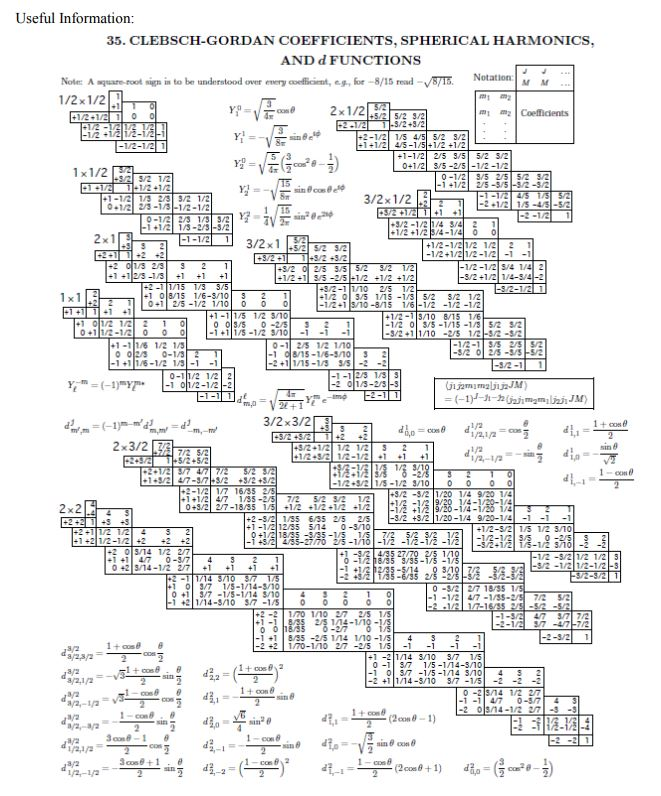
\includegraphics[width=\textwidth]
		{images/TCG.png}
		\caption{\label{fig:my-label} Tavole di C-G con annesse armoniche sferiche}}
\end{figure}


Ovviamente tutto questo discorso ci permette di ricavare informazioni per ogni momento angolare composto, che sia esso orbitale $L=l_1+l_2$, di spin $S=s_1+s_2$ o totale $J= L+S$


\newpage

\subsection{Stati di singoletto e tripletto}

Un caso molto interessante di composizione dei momenti riguarda quello degli spin degli elettroni.

Presi due elettroni con
\begin{align}
&s_1=\frac{1}{2}=s_2 \\
&s_z=\pm \frac{1}{2}
\end{align}

Nella base $\ket{s_{z_1},s_{z_2}}$ avremo quattro possibilità:
\begin{align}
\ket{+,+} \quad;\quad \ket{+,-} \quad;\quad \ket{-,+} \quad;\quad \ket{-,-}
\end{align}

Invece nella base $\ket{S_T,S_{T_z}}$ avremo che
\begin{align}
{}& s_1-s_2 \leq S_T \leq s_1+s_2 \rightarrow S_T=0,1 \; ;\; S_{T_z}=0,\pm 1 \\
& \ket{1,+1} \quad;\quad \ket{1,0} \quad;\quad \ket{1,-1} \quad;\quad \ket{0,0}
\end{align}

dove avremo gli stati simmetrici rispetto allo scambio di elettroni
\begin{align}
{}&\ket{1,+1} = \ket{+,+} \\
&\ket{1,-1} = \ket{-,-} \\
\end{align}

Come troviamo $\ket{1,0}$? Immaginiamo di applicare a $\ket{1,+1}$ l'operatore di discesa $S_-= S_x - iS_y$. 

Lo stato $\ket{1,+1= }\ket{+,+}$ è però \textbf{simmetrico allo scambio di elettroni} e anche l'operatore $S_-=s_{1_-}+s_{2_-}$ lo è, quindi anche $S_-\ket{+,+}$ lo sarà. Questo vuol dire che la combinazione di $\ket{+,-}$ e di $\ket{-,+}$ dovrà esserlo, e l'unica possible sarà
\begin{align}
&\ket{1,0} = \frac{1}{\sqrt{2}}(\ket{+,-} + \ket{-,+})
\end{align}

E abbiamo così trovato gli stati simmetrici detti di \textbf{tripletto}, mentre quello di \textbf{singoletto} sarà l'unica combinazione ortogonale rimasta, ovvero l'antisimmetrica:
\begin{align}
&\ket{0,0} = \frac{1}{\sqrt{2}}(\ket{+,-} - \ket{-,+})
\end{align}

\newpage

\section{L'operatore di scambio e il principio di Pauli}

Il discorso del P.d.P. nasce dal fatto che, presi due elettroni, se il problema si studia solo spazialmente essi sono indistinguibili.

Prendiamo un sistema composto dai suddetti:
\begin{align}
\ket{q,p,s}_1 \quad;\quad \ket{q,p,s}_2
\end{align}

Se queste sono davvero identiche deve essere per forza che \textbf{le funzioni associate devono essere simmetriche per scambio di particelle}, altrimenti avremmo un assurdo.

Introduciamo quindi l'\textbf{operatore di scambio} $\Pi$:
\begin{align}
\left\{
\begin{array}{cc}
\Pi q_1\Pi^{-1}=q_2 \\
\Pi q_2\Pi^{-1}=q_1
\end{array}
\right.
\quad ; \quad
\left\{
\begin{array}{cc}
\Pi p_1\Pi^{-1}=p_2 \\
\Pi p_2\Pi^{-1}=p_1
\end{array}
\right.
\quad ; \quad
\left\{
\begin{array}{cc}
\Pi s_1\Pi^{-1}=s_2 \\
\Pi s_2\Pi^{-1}=s_1
\end{array}
\right.
\end{align}

Si può anche dire che l'indistinguibilità delle particelle si traduce nel fatto che tutte le osservabili del sistema commutano con $\Pi$.

Per il \textbf{th. di Von Neumann} sappiamo che l'operatore associato a $\Pi$ è unico e unitario, e quindi
\begin{align}
\Pi\ket{A,B}=e^{i\phi}\ket{B,A}
\end{align}
poniamo
\begin{align}
{}&\Pi^2=1\\
&\Pi^{-1}=\Pi^\dagger=\Pi
\end{align}

Da cui segue che, chiamati gli stati \textbf{simmetrici} $\ket{S}$ e quelli \textbf{antisimmetrici} $\ket{A}$ gli unici autovalori possibili sono
\begin{align}
{}&\Pi\ket{S} = +1\ket{S} \\
&\Pi\ket{A} = -1\ket{A}
\end{align}

Una volta definiti questi due tipi di stati possiamo riscrivere tutti gli stati come combinazione di questi due tipi. In altre parole tutti gli stati vivono in uno spazio dato da
\begin{align}
H=H_S \otimes H_A
\end{align}

Qualora uno stato viva solo in uno dei due vi rimane per sempre.

\subsection{Principio di Pauli}

Se consideriamo l'atomo di elio e ci concentriamo sull'orbitale, sappiamo sperimentalmente che tale sistema è desritto dallo stato
\begin{align}
\ket{1s^2;S=0}
\end{align}
mentre è impossibile avere
\begin{align}
\ket{1s^2;S=1}
\end{align}

che in teoria sarebbe uno stato possibile. Questa evidenza sperimentale ci porta a due conseguenze:

\begin{enumerate}
	\item non tutti gli stati di $H$ rappresentano stati fisici 
	\item preso un sistema di due elettroni, l'unico stato possibile è quello antisimmetrico.
\end{enumerate}

Definite ora le famiglie di particelle

\begin{enumerate}
	\item \textbf{Fermioni}: particelle a spin semintero (elettroni, protoni, neutroni,...)
	\item \textbf{Bosoni}: particelle a spin intero (mesoni $\pi$,...)
\end{enumerate}

possiamo enunciare il \textbf{Principio di Pauli per il caso fermionico}:

\textit{Preso un sistema di due o più fermioni, gli unici stati possibili sono quelli rappresentati da vettori antisimmetrici rispetto allo scambio di una qualunque coppia di fermioni.}

Per il \textbf{caso bosonico} il discorso è analogo, ma gli stati sono invece \textbf{simmetrici}.

\newpage

Notiamo come per il princio di Pauli il numero di stati per un sistema a particelle identiche sia minore di quello per un sistema a particelle indistinguibili, infatti

\begin{enumerate}
	\item $e^+ \quad;\quad e^-$
	\begin{enumerate}
		\item $\ket{A}_+ \ket{B}_-$
		\item $\ket{B}_+ \ket{A}_-$
	\end{enumerate}
	
	\item $e^- \quad;\quad e^-$
	\begin{enumerate}
		\item $\ket{A}_-\ket{B}_- - \ket{B}_-\ket{A}_-$
	\end{enumerate}
\end{enumerate}

Il che si traduce anche nel dire che \textbf{un sistema a particelle identiche non è mai a variabili separabili e i suoi stati non sono mai fattorizzati}.

Il P.d.P. spiega anche perché gli orbitali possono ospitare al massimo due elettroni, in quanto \textbf{è impossibile creare uno stato di spin di tre o più elettroni antisimmetrico rispetto allo scambio dei numeri di spin di ogni coppia}:

\begin{enumerate}
	\item $\ket{+,+,+} \quad;\quad \ket{-,-,-}$
	
	Questi stati sono totalmente simmetrici
	
	\item $\ket{+,+,-} \quad;\quad \ket{+,-,+} \quad;\quad \ket{-,+,+}\quad;\quad \ket{-,-,+}\quad;\quad \ket{-,+,-}\quad;\quad \ket{+,-,-}$
	
	Questi stati sono simmetrici rispetto ad uno scambio e nessuna combinazione sarà mai completamente antisimmetrica
\end{enumerate}

Un'altra interessante questione deriva dal fatto che \textbf{tutte le informazioni relative alle proprietà di uno stato sono contenute nella collezione dei valori medi delle osservabili}

\begin{enumerate}
	\item \textbf{Particelle distinguibili:} $\ket{X}=\ket{A_1,B_2}$
	\begin{align}
	\braket{X|\xi|X}= \braket{A_1,B_2|\xi|A_1,B_2}
	\end{align}
	
	\item \textbf{Particelle indistinguibili:} $\ket{Y}=\frac{1}{\sqrt{2}}(\ket{A_1,B_2} \pm \ket{B_1,A_2})$	
		\begin{align}
		\braket{Y|\xi|Y} {}&= \frac{1}{2}(\bra{A_1,B_2} \pm \bra{B_1,A_2})\xi(\ket{A_1,B_2} \pm \ket{B_1,A_2}) = \nonumber \\
		&= \frac{1}{2}(\braket{A_1,B_2 |\xi| A_1,B_2} + \braket{B_1,A_2 |\xi| B_1,A_2}) + \nonumber \\
		&\quad + \frac{1}{2}(\pm \braket{A_1,B_2 |\xi| B_1,A_2} \pm \braket{B_1,A_2 |\xi| A_1,B_2})
		\end{align}
		ma dato che 
		\begin{align}
		\left\{
		\begin{array}{cc}
		\Pi=\Pi^{-1} \\
		\Pi\ket{A,B}=\ket{B,A}
		\end{array}		
		\right. 
		\end{align}
		avremo 
		\begin{align}	
		\braket{B_1,A_2|\xi|B_1,A_2}=\braket{B_1,A_2|\Pi^\dagger\xi\Pi|B_1,A_2}= \braket{A_1,B_2|\xi|A_1,B_2} \\
		\braket{B_1,A_2|\xi|A_1,B_2}= \braket{B_1,A_2|\Pi^\dagger\xi\Pi|A_1,B_2}= \braket{A_1,B_2|\xi|B_1,A_2}
		\end{align}
		da cui
		\begin{align}
		\braket{Y|\xi|Y} = \braket{A_1,B_2 |\xi| A_1,B_2} \pm \braket{A_1,B_2 |\xi| B_1,A_2}
		\end{align}
				
		Il secondo termine viene detto \textbf{di interferenza}, e il segno dipende dal tipo di particella (fermioni o bosoni).
\end{enumerate}

Notiamo che un sistema di particelle identiche con termine di interferenza nullo si tratta esattamente come un sistema di particelle indistinguibili. Questo spiega perché quando si studia un singolo atomo (per esempio H) non è necessario considerare gli altri elettroni nel sistema universo. 

Infatti se due sistemi descritti dagli stati $\ket{A}$ e $\ket{B}$ \textbf{sono lontani e localizzati} e quindi le loro funzioni d'onda $\psi_A(x)$ e $\psi_B(x)$ hanno \textbf{supporti disgiunti}, il termine di interferenza si annulla e si possono studiare i sottosistemi indipendentemente.

Il discorso è lo stesso anche  in caso di rappresentazione degli impulsi, in quanto
\begin{align}
p=-i \hbar \frac{\partial}{\partial x}
\end{align}

E i supporti delle derivate sono gli stessi delle funzioni di partenza. 